\section{Shelf Localization and Base Movement}
\label{sec:shelf}

As described in Sec.~\ref{sec:platform}, we used a PR2 as our robot platform. Since the arms' reachability of PR2 is relatively small in comparison to the shelf size, it is not feasible to define a fixed location for the robot to achieve the required task. As such, we have to exploit the mobility to enlarge the working space, so that the robot would be able to reach and grasp from most of the shelf bins, as well as loading the grasped objects into the order bin.

For this, shelf localization, which serves as the only landmark in the workcell, is essential for our system to guide the robot navigating between different grasping positions. Since the robot movement accumulates localization errors, it is necessary to localize the shelf in real time to close the control loop for base movement. 

\begin{figure}[htb]
\centering
	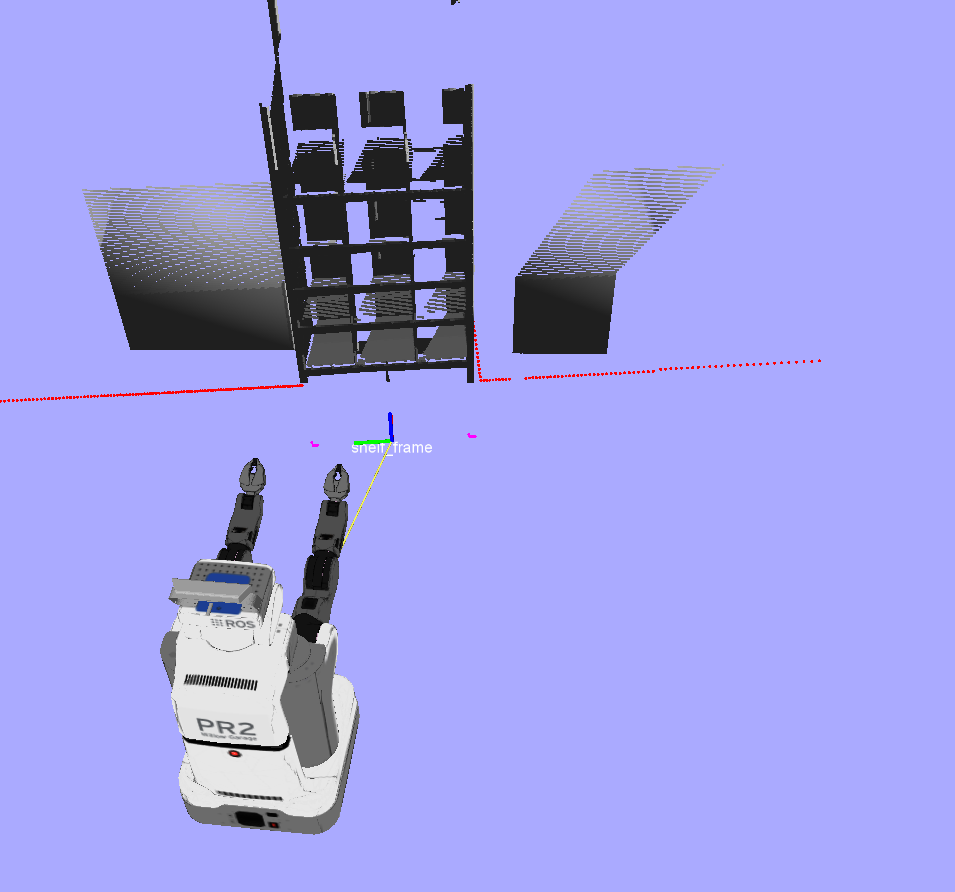
\includegraphics[height=0.39\columnwidth]{figures/localization.png}
	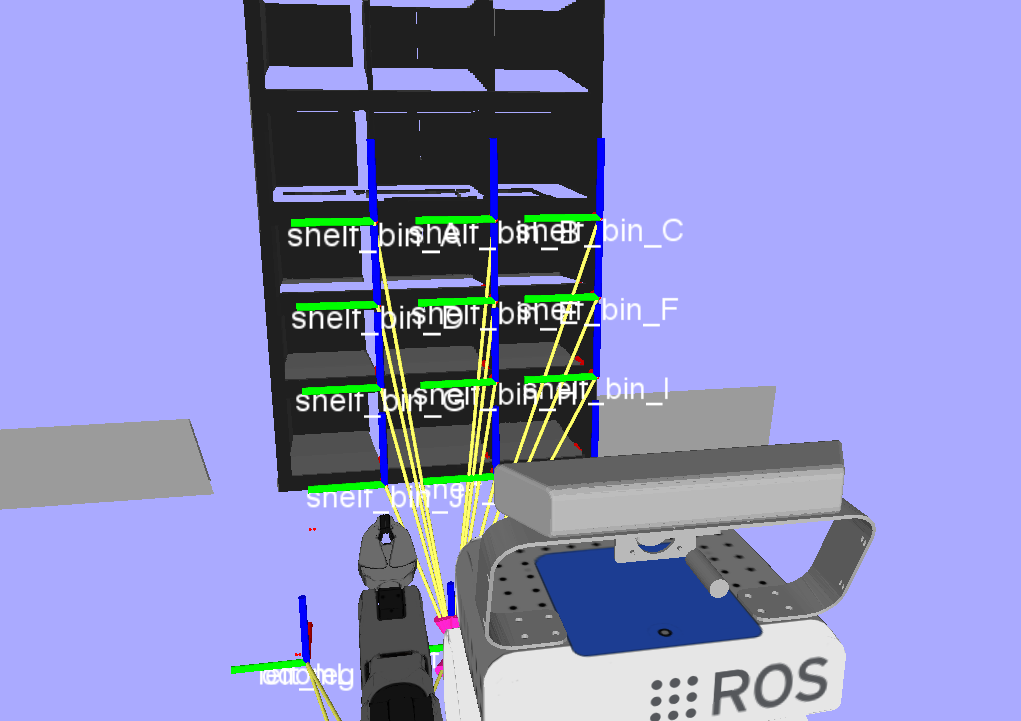
\includegraphics[height=0.39\columnwidth]{figures/binFrames.png}
        \caption{\emph{Left}: An example of shelf localization shown in rviz. The x and y coordinates of shelf\_frame is defined as the center of two front legs, while the height of it is the same as the base\_laser\_link. \emph{Right}: The bin frames are located at the right bottom corner of each bin.}
        \label{fig:localization}
\end{figure}

As shown in Fig.~\ref{fig:localization}, we use the base laser scanner to localize the two front legs of the shelf. Observing that the shelf is located in front of the robot, where no any other objects are close by. Therefore, it is reasonable to find the closest point cluster and consider it as one of the legs, while the remaining cluster is considered as another leg. However, this is not a reliable procedure as there could be noise or other unexpected objects, e.g., human legs. As such, our shelf localization consists of two procedures as follows:

\begin{itemize}
 \item \textbf{Detection:} Once the front legs are detected, before the system starts to autonomously work on assigned tasks, a human supervisor needs to confirm to the robot that the detection is correct. In case when the detection is incorrect, we need to clear the occlusions in front of the shelf until a confirmation is made.
 \item \textbf{Tracking:} While the robot is moving, given that we know the motion model of the robot, we update the shelf localization using a Kalman filter.
\end{itemize}

Having localized the shelf, we further estimate the shelf bin frames based on the known mesh model, see Fig.~\ref{fig:localization}. As will be described in Sec.~\ref{fig:localization}, knowing the bin frames will facilitate the grasp planning in our system.